
%--------------------------------------------------------------------
%                            Preample
%--------------------------------------------------------------------

\documentclass[aspectratio=1610,17pt,utf8]{beamer}

\usepackage[utf8]{inputenc}
\usepackage[T1]{fontenc}
\usepackage[USenglish]{babel}
\usepackage{graphicx} % graphics
\usepackage{mathabx}
\usepackage{mathpazo}
\usepackage{eulervm}


% title slide definition
\title[DS]{Distributed Systems}
\subtitle{Exam}
\author[Thomas Møller Jensen]{Thomas Møller Jensen}
\institute[Institute of Computer Science]
{
  Aalborg University\\
}

%--------------------------------------------------------------------
%                            Titlepage
%--------------------------------------------------------------------

\begin{document}

%-------------------------------------------------------------------
%                            Content
%-------------------------------------------------------------------
%                 Distributed Mutual Exclusion
%-------------------------------------------------------------------

\begin{frame}{Distributed Mutual Exclusion}
    What is a mutex? Kinda a Lock for distributed systems...

    In a distributed system a mutex is for locking a shared resource in a network, traditionally in a program, a lock would be enough to handle concurrent writes/reads, but when the communication is expensive, locking the resource is harder to do.
\end{frame}

\begin{frame}{Mutex Algorithms}
    \section{Mutex algorithms}
    \begin{itemize}
        \item Centralized approach
        \item Token Ring
        \item Ricart and Agrawala's algorithm
            \begin{itemize} 
                \item Lamport Clocks
            \end{itemize}
    \end{itemize}
\end{frame}

\begin{frame}{Centralized algortihm}
    \begin{minipage}{.45\textwidth}
        \begin{figure}
            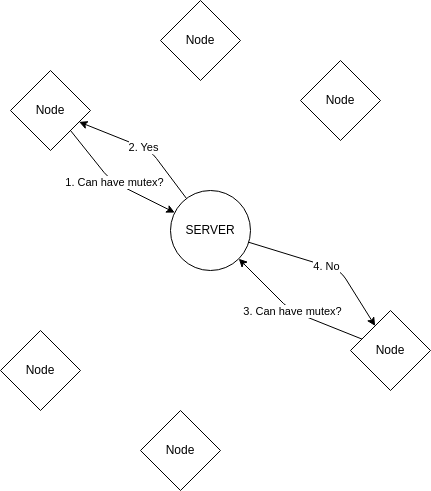
\includegraphics[width=\textwidth]{figures/mutex.png}
        \end{figure}
    \end{minipage}
    \begin{minipage}{.5\textwidth}
        \tiny{All three nodes highlighted are points of failure}
    \end{minipage}
\end{frame}

%-------------------------------------------------------------------
%                 Multicast/Group Communication
%-------------------------------------------------------------------

\begin{frame}{Multicast/Group Communication}
\end{frame}

%-------------------------------------------------------------------
%                     Consensus Protocols
%-------------------------------------------------------------------

\begin{frame}{Consensus Protocols}
\end{frame}

%-------------------------------------------------------------------
%                 Replication and Consistency
%-------------------------------------------------------------------

\begin{frame}{Replication and Consistency}
\end{frame}

%-------------------------------------------------------------------
%                     Distributed Storage
%-------------------------------------------------------------------

\begin{frame}{Distributed Storage}
\end{frame}

%-------------------------------------------------------------------
%                     Big Data Analytics
%-------------------------------------------------------------------

\begin{frame}{Big Data Analytics}
\end{frame}

%-------------------------------------------------------------------
%                         Blockchains
%-------------------------------------------------------------------

\begin{frame}{Blockchains}
\end{frame}

%-------------------------------------------------------------------
%                  Peer-to-Peer Networking
%-------------------------------------------------------------------

\begin{frame}{Peer-to-Peer Networking}
\end{frame}

%-------------------------------------------------------------------
%              Internet of Things and Routing
%-------------------------------------------------------------------

\begin{frame}{Internet of Things and Routing}
\end{frame}

\end{document}